\documentclass[10pt,border=3pt]{standalone}
\usepackage{mathptmx}
\usepackage{tikz}
\usetikzlibrary{arrows.meta,fit,backgrounds,calc,positioning}
\definecolor{acc}{HTML}{0B5394}
\definecolor{accl}{HTML}{EAF0F7}
\definecolor{grp}{HTML}{F5F5F5}
\tikzset{
 box/.style={draw=black,line width=0.6pt,fill=white,rounded corners=1.5pt,align=center,font=\small,inner sep=2pt},
 gbox/.style={box,draw=acc,line width=0.8pt},
 cont/.style={draw=black!50,line width=0.5pt,rounded corners=3pt,fill=grp,inner xsep=5pt,inner ysep=5pt},
 gcont/.style={draw=acc,line width=0.8pt,rounded corners=3pt,fill=accl,inner xsep=5pt,inner ysep=5pt},
 ttl/.style={font=\normalsize\bfseries,anchor=west,inner sep=0pt},
 arr/.style={-{Latex[length=2.4mm,width=1.8mm]},line width=0.7pt},
 ln/.style={line width=0.7pt},
 num/.style={circle,draw=black,fill=white,font=\footnotesize\bfseries,inner sep=0pt,minimum size=4.4mm,anchor=west}
}
% box(name, cx, cy, width, height, style, text)
\newcommand{\B}[7]{\node[#6,text width=#4cm-4pt,minimum height=#5cm] (#1) at (#2,#3) {#7};}
\newcommand{\T}[4]{\node[num,#4] (n#1) at (#2) {#1}; \node[ttl,#4,right=3pt of n#1] (t#1) {#3};}
\begin{document}
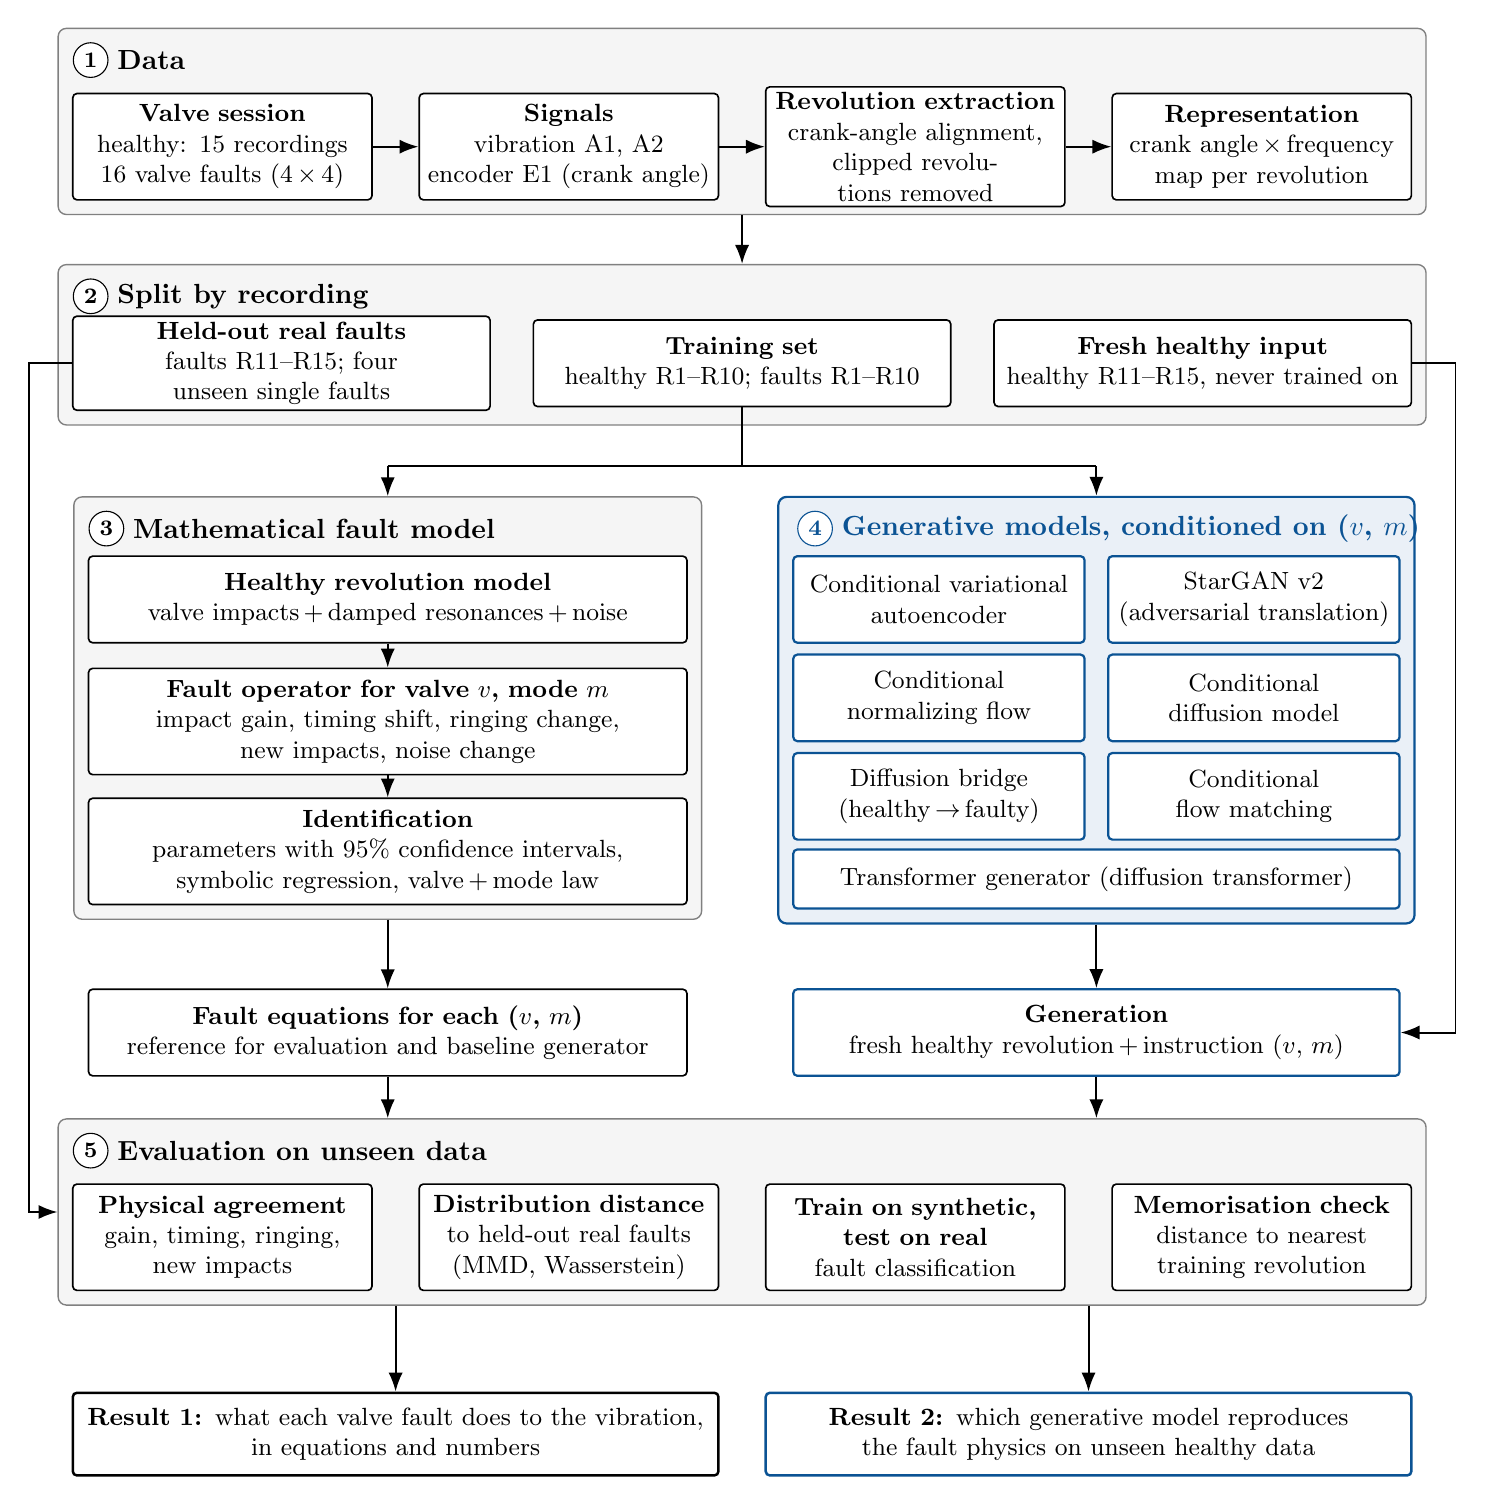
\begin{tikzpicture}
% ===== 1 Data (y = 0)
\B{d1}{1.9}{0}{3.8}{1.35}{box}{\textbf{Valve session}\\ healthy: 15 recordings\\ 16 valve faults (4\,$\times$\,4)}
\B{d2}{6.3}{0}{3.8}{1.35}{box}{\textbf{Signals}\\ vibration A1, A2\\ encoder E1 (crank angle)}
\B{d3}{10.7}{0}{3.8}{1.35}{box}{\textbf{Revolution extraction}\\ crank-angle alignment,\\ clipped revolutions removed}
\B{d4}{15.1}{0}{3.8}{1.35}{box}{\textbf{Representation}\\ crank angle\,$\times$\,frequency\\ map per revolution}
\foreach \a/\b in {d1/d2,d2/d3,d3/d4} \draw[arr] (\a) -- (\b);
\T{1}{0,1.1}{Data}{}
\begin{scope}[on background layer]\node[cont,fit=(n1)(d1)(d4)] (c1) {};\end{scope}
% ===== 2 Split (y = -2.75)
\B{s1}{2.65}{-2.75}{5.3}{1.1}{box}{\textbf{Held-out real faults}\\ faults R11--R15; four unseen single faults}
\B{s2}{8.5}{-2.75}{5.3}{1.1}{box}{\textbf{Training set}\\ healthy R1--R10; faults R1--R10}
\B{s3}{14.35}{-2.75}{5.3}{1.1}{box}{\textbf{Fresh healthy input}\\ healthy R11--R15, never trained on}
\T{2}{0,-1.9}{Split by recording}{}
\begin{scope}[on background layer]\node[cont,fit=(n2)(s1)(s3)] (c2) {};\end{scope}
\draw[arr] (c1.south -| s2) -- (c2.north -| s2);
% ===== 3 Mathematical model (left) and 4 Generative models (right), top y = -5.05
\B{m1}{4.0}{-5.75}{7.6}{1.1}{box}{\textbf{Healthy revolution model}\\ valve impacts\,+\,damped resonances\,+\,noise}
\B{m2}{4.0}{-7.3}{7.6}{1.35}{box}{\textbf{Fault operator for valve $v$, mode $m$}\\ impact gain, timing shift, ringing change,\\ new impacts, noise change}
\B{m3}{4.0}{-8.95}{7.6}{1.35}{box}{\textbf{Identification}\\ parameters with 95\% confidence intervals,\\ symbolic regression, valve\,+\,mode law}
\draw[arr] (m1) -- (m2); \draw[arr] (m2) -- (m3);
\T{3}{0.2,-4.85}{Mathematical fault model}{}
\begin{scope}[on background layer]\node[cont,fit=(n3)(m1)(m3)] (c3) {};\end{scope}
\B{g1}{11.0}{-5.75}{3.7}{1.1}{gbox}{Conditional variational\\ autoencoder}
\B{g2}{15.0}{-5.75}{3.7}{1.1}{gbox}{StarGAN v2\\ (adversarial translation)}
\B{g3}{11.0}{-7.0}{3.7}{1.1}{gbox}{Conditional\\ normalizing flow}
\B{g4}{15.0}{-7.0}{3.7}{1.1}{gbox}{Conditional\\ diffusion model}
\B{g5}{11.0}{-8.25}{3.7}{1.1}{gbox}{Diffusion bridge\\ (healthy\,$\to$\,faulty)}
\B{g6}{15.0}{-8.25}{3.7}{1.1}{gbox}{Conditional\\ flow matching}
\B{g7}{13.0}{-9.3}{7.7}{0.75}{gbox}{Transformer generator (diffusion transformer)}
\node[num,draw=acc,text=acc] (n4) at (9.2,-4.85) {4};
\node[ttl,text=acc,right=3pt of n4] (t4) {Generative models, conditioned on ($v$, $m$)};
\begin{scope}[on background layer]\node[gcont,fit=(n4)(g1)(g2)(g7)] (c4) {};\end{scope}
% training bus
\draw[ln] (s2.south) -- ++(0,-0.75) coordinate (bus);
\draw[ln] (4.0,0|-bus) -- (13.0,0|-bus);
\draw[arr] (4.0,0|-bus) -- (4.0,0|-c3.north);
\draw[arr] (13.0,0|-bus) -- (13.0,0|-c4.north);
% ===== row 4: equations (left) and generation (right)
\B{q}{4.0}{-11.25}{7.6}{1.1}{box}{\textbf{Fault equations for each ($v$, $m$)}\\ reference for evaluation and baseline generator}
\B{gen}{13.0}{-11.25}{7.7}{1.1}{gbox}{\textbf{Generation}\\ fresh healthy revolution\,+\,instruction ($v$, $m$)}
\draw[arr] (c3.south -| q) -- (q.north);
\draw[arr] (c4.south -| gen) -- (gen.north);
\draw[arr] (s3.east) -- ++(0.55,0) |- (gen.east);
% ===== 5 Evaluation
\B{e1}{1.9}{-13.85}{3.8}{1.35}{box}{\textbf{Physical agreement}\\ gain, timing, ringing,\\ new impacts}
\B{e2}{6.3}{-13.85}{3.8}{1.35}{box}{\textbf{Distribution distance}\\ to held-out real faults\\ (MMD, Wasserstein)}
\B{e3}{10.7}{-13.85}{3.8}{1.35}{box}{\textbf{Train on synthetic,}\\ \textbf{test on real}\\ fault classification}
\B{e4}{15.1}{-13.85}{3.8}{1.35}{box}{\textbf{Memorisation check}\\ distance to nearest\\ training revolution}
\T{5}{0,-12.75}{Evaluation on unseen data}{}
\begin{scope}[on background layer]\node[cont,fit=(n5)(e1)(e4)] (c5) {};\end{scope}
\draw[arr] (q.south) -- (q.south |- c5.north);
\draw[arr] (gen.south) -- (gen.south |- c5.north);
\draw[arr] (s1.west) -- ++(-0.55,0) |- (c5.west);
% ===== results
\B{r1}{4.1}{-16.35}{8.2}{1.05}{box,line width=0.9pt}{\textbf{Result 1:} what each valve fault does to the vibration,\\ in equations and numbers}
\B{r2}{12.9}{-16.35}{8.2}{1.05}{gbox,line width=0.9pt}{\textbf{Result 2:} which generative model reproduces\\ the fault physics on unseen healthy data}
\draw[arr] (c5.south -| r1) -- (r1.north);
\draw[arr] (c5.south -| r2) -- (r2.north);
\end{tikzpicture}
\end{document}
